% document style header
\documentclass[a4paper, 12pt]{config/homework}

% import default packages
\usepackage{config/packages}
\usepackage{config/commands}
\DeclareSIUnit{\atm}{atm}

% end preamble
\begin{document}

% document title
\noindent
\hfill Calvin Sprouse \hfill PHYS 475 Homework 2 \hfill 2024 April 10 \hfill
\bigskip

% homework problems begin
% Textbook problems 1.27, 1.28, 1.29, 1.31, 1.33, 1.35, 1.37, 1.41, 1.42
\bigskip\noindent \textbf{Problem 1.27.}
Give an example of a process in which no heat is added to a system, but its temperature increases. Then give an example of the opposite: a process in which heat is added to a system but its temperature does not change.

\bigskip\noindent
Any system undergoing non-isothermal compression will experience a temperature increase without the addition of heat. When a system is allowed to expand, any addition of heat will cause an increase in volume while the temperature remains constant.

\bigskip\noindent \textbf{Problem 1.28.}
Estimate how long it should take to bring a cup of water to boiling temperature in a typical 600-watt microwave oven, assuming that all the energy ends up in the water. Assume any reasonable initial temperature for the water. Explain why no heat is involved in this process.

\bigskip\noindent
Let the water be at room temperature, \(T_i = \qty{293}{\kelvin}\), before the microwave is turned on. The energy required to raise the temperature of water by some amount is given by
\[E = m c \Delta T = V\left(\qty{1}{\gram\per\milli\liter}\right)\left(\qty{4.182}{\joule\per\gram\per\kelvin}\right)\left(\qty{80}{\kelvin}\right),\]
where the mass of the water is represented by the volume and density, \(c\) is the specific heat capacity of water, and \(\Delta T\) is the temperature difference in kelvin between the boiling temperature of water and room temperature. Let
\[V=1\,\text{cup}\approx\qty{250}{\milli\liter}.\]
Then,
\[E = \qty{8.364e4}{\joule}.\]
The time required to deliver an amount of energy \(E\) at some wattage \(W\) is given by
\[t = \frac{E}{W} = \frac{\qty{8.364e4}{\joule}}{\qty{600}{\joule\per\second}} = \qty{139.4}{\second}.\]
The microwave should bring a cup of room temperature water to boil in 139.4 seconds. There is no heat involved in this process. Heat is defined as the spontaneous flow of energy between two objects of different temperature. The microwave, however, is not transferring energy on the basis of a temperature gradient. The microwave transfers energy through directed radiation.


% \bigskip\noindent
\pagebreak\noindent
\textbf{Problem 1.29.} Put a few spoonfuls of water into a bottle with a tight lid. Make sure everything is at room temperature, measuring the temperature of the water with a thermometer to make sure. Now close the bottle and shake it as hard as you can for several minutes. When you're exhausted and ready to drop, shake it for several minutes more. Then measure the temperature again. Make a rough calculation of the expected temperature change, and compare.

\bigskip\noindent
Suppose we have a water bottle which will absorb a negligible amount of heat from the water and be of negligible mass. The water then shall be of mass \(m\). Let the water start at room temperature, \(T_i=\qty{293}{\kelvin}\). The final temperature of the water then, after receiving some heat energy \(Q\), is given by
\[T_f = \frac{Q}{mc} + T_i.\]
Now suppose the water bottle is shaken upward violently, a height \(h\). The water gains some potential gravitational energy, which will be lost in the downward motion and so can be ignored, but the violence of the shake means there exists some additional kinetic energy. This kinetic energy is not used to raise the water higher in the gravitational potential, but is instead lost to chaotic motion of the water in the bottle. If we imagine the shaker lost grip and simply tossed the bottle into the air, then the difference in potential energy of the bottle tossed vs.\ the bottle held is the extra energy the water receives from violent shaking. Suppose the shaker could toss the bottle upward a height \(H\), where \(H>h\). Then the extra kinetic energy of the water after the upward shake is given by
\[K = mg\left(H-h\right).\]
On the downward shake now, we suppose the shaker can impart a similar amount of energy. Then over one shake cycle, the shaker imparts kinetic energy to the water
\[K = 2mg\left(H-h\right).\]
As the water settles, this kinetic energy of the water molecules becomes thermal energy of the water. Suppose all this kinetic energy becomes thermal energy of the water. Then one shake cycle should raise the temperature of water by
\[T_f = \frac{2mg\left(H-h\right)}{mc} + T_i = \frac{2g}{c}\left(H-h\right) + T_i.\]
We see that the mass of the water has no effect, though I'm sure the shaker's arm would disagree. If we shake the water for \(N\) cycles, the final temperature should be
\[T_f = N\frac{2g}{c}\left(H-h\right) + T_i.\]
Now, suppose a shaker can toss a bottle of water a height \(H=\qty{3}{\meter}\) and the same bottle is shaken through a height \(h=\qty{1}{\meter}\). To reach boiling temperature, \(T_f = \qty{373}{\kelvin}\), would require \(N\) shakes given by
\[N = \frac{c\left(T_f-T_i\right)}{H-h}.\]
Substituting our hypothetical values yields
\[N= 167,280.\]
Unfortunately, this is a best case scenario. Much of the energy the shaker puts into the water will be lost to sound and to the shakers own muscles stopping the bottle at the top and bottom of the shake.

% \bigskip\noindent
\pagebreak\noindent
\textbf{Problem 1.31.} Imagine some helium in a cylinder which an initial volume of 1 liter and an initial pressure of 1 atm. Somehow, the helium is made to expand to a final volume of 3 liters, in such a way that its pressure rises in direct proportion to its volume.
\begin{enumerate}[label=\textbf{(\alph*)}]
\item Sketch a graph of pressure vs.\ volume for this process.

\begin{figure}[H]
\centering
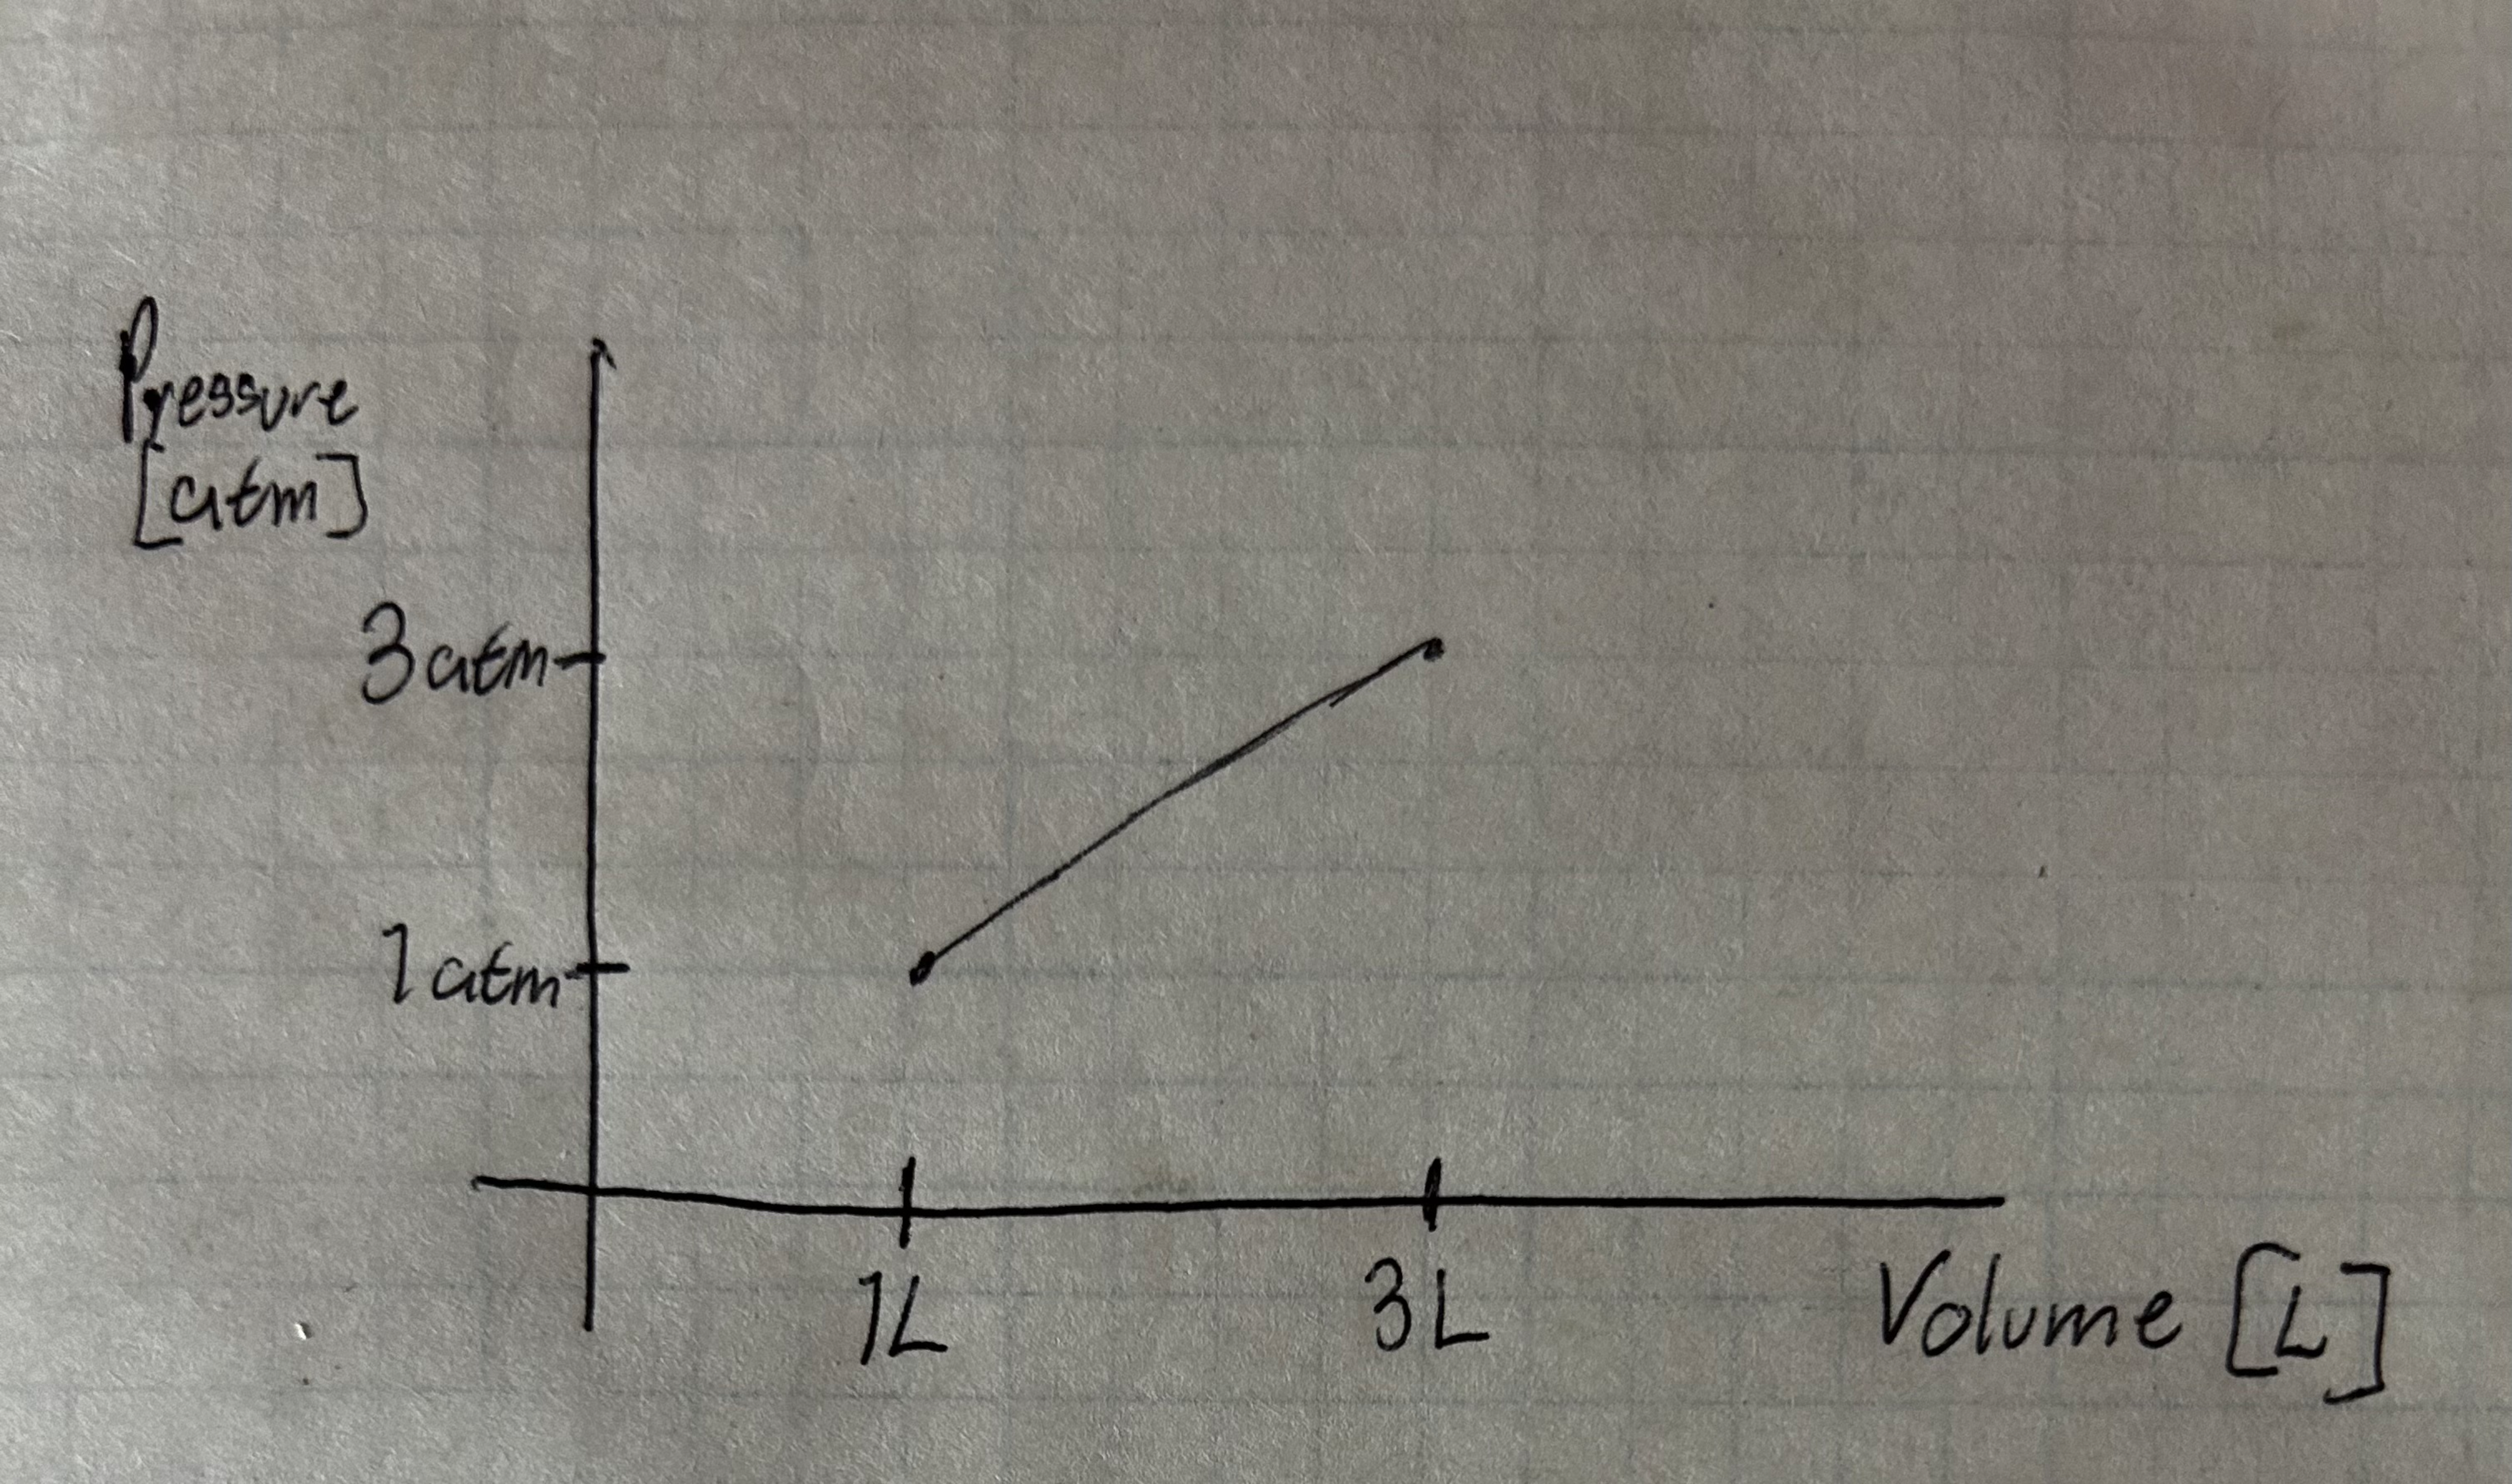
\includegraphics[width=0.5\textwidth]{figure.pdf}
\end{figure}

\item Calculate the work done on the gas during this process, assuming that there are are no ``other'' types of work being done.

The area under the curve is given by
\[W = \frac{1}{2}\left(\qty{3}{\atm}\right)\left(\qty{3}{\liter}\right) = \qty{4.5}{\joule}.\]

\item Calculate the change in the helium's energy content during this process.

\[\Delta E = P_f V_f - P_i V_i = \left(\qty{3}{\atm}\right)\left(\qty{3}{\liter}\right) - \left(\qty{1}{\atm}\right)\left(\qty{1}{\liter}\right) = \qty{8}{\joule}.\]

\item Calculate the amount of heat added to or removed from the helium during this process.

Since only \(\qty{4.5}{\joule}\) of energy was added through work, the remaining \(\qty{3.5}{\joule}\) of energy must come from heat.

\item Describe what you might do to \textit{cause} the pressure to rise as the helium expands.

As the gas expands I might heat it to replenish the energy lost to expansion.
\end{enumerate}

\bigskip\noindent


% \bigskip\noindent
\pagebreak\noindent
\textbf{Problem 1.33.} An ideal gas is made to undergo the cyclic process shown in Figure 1.10(a). For each of the steps \(A\), \(B\), and \(C\), determine whether each of the following is positive, negative, or zero:
\begin{enumerate}[label=(\alph*)]
\item the work done on the gas;
\item the change in the energy content of the gas;
\item the heat added to the gas.
\end{enumerate}
Then determine the sign of each of these three quantities for the whole cycle. What does this process accomplish?

\bigskip\noindent
% generate a 4x4 table
\begin{center}
\begin{tabular}{c|c|c|c}
& (a) Work & (b) Energy & (c) Heat \\ \hline \hline
A & - & - & 0 \\ \hline
B & 0 & + & + \\ \hline
C & + & + & 0 \\ \hline \hline
cycle & 0 & + & + \\ \hline
\end{tabular}
\end{center}

\noindent
This process increases the energy of the gas.

\bigskip\noindent \textbf{Problem 1.35.} Derive equation 1.40,
\[V^\gamma P = \text{constant},\]
from equation 1.39,
\[VT^{f/2} = \text{constant}.\]
\bigskip\noindent
We begin with Eq.\ 1.38,
\[V_\text{f}T_\text{f}^{f/2} = V_\text{i}T_\text{i}^{f/2}.\]
Then, solving the ideal gas law for \(T\) yields
\[T = \frac{PV}{nR}.\]
Substituting this relation and recognizing that \(nR\) is constant yields
\[V_\text{f}\left(\frac{P_\text{f}V_\text{f}}{nR}\right)^{f/2} = V_\text{i}\left(\frac{P_\text{i}V_\text{i}}{nR}\right)^{f/2}.\]
Multiplying both sides by \(nR\) and combining the exponents yields
\[P_\text{f}V_\text{f}^{\frac{f+2}{2}} = P_\text{i}V_\text{i}^{\frac{f+2}{2}} \Rightarrow PV^\gamma = \text{constant}.\]


% \bigskip\noindent
\pagebreak\noindent
\textbf{Problem 1.37.} In a Diesel engine, atmospheric air is quickly compressed to about \(1/20\) of its original volume. Estimate the temperature of the air after compression, and explain why a Diesel engine does not require spark plugs.

\bigskip\noindent
Let the gas be at room temperature before compression, \(T_i = \qty{293}{\kelvin}\), and let the volume of the gas before compression be \(V\). Then, Eq.\ 1.38 states
\[V_\text{f}T_\text{f}^{f/2} = V_\text{i}T_\text{i}^{f/2},\]
where \(f\) is the number of degrees of freedom of the gas. Since air is composed almost entirely of diatomic molecules \(\text{O}_2\) and \(\text{N}_2\), \(f=5\). Then,
\[T_\text{f} = \left(\frac{V_i}{V_f}\right)^{2/f} T_\text{i} = (20)^{2/5}\qty{293}{\kelvin} \approx \qty{971}{\kelvin}.\]
This temperature is presumably higher than the auto-ignition temperature of Diesel fuel thus allowing the engine to create combustion without the need for a spark.

% \bigskip\noindent
\pagebreak\noindent
\textbf{Problem 1.41.} To measure the heat capacity of an object, all you usually have to do is put it in thermal contact with another object whose heat capacity you know. As an example, suppose that a chunk of metal is immersed in boiling water \((\qty{100}{\celsius})\), then is quickly transferred into a Styrofoam cup containing \(\qty{250}{\gram}\) of water at \(\qty{20}{\celsius}\). After a minute or so, the temperature of the contents of the cup is \(\qty{24}{\celsius}\). Assume that during this time no significant energy is transferred between the contents of the cup and the surroundings. The heat capacity of the cup itself is negligible.
\begin{enumerate}[label=\textbf{(\alph*)}]
\item How much heat is gained by the water?

The water gains heat \(Q\).
\item How much heat is lost by the metal?

The metal loses heat \(Q\).
\item What is the heat capacity of this chunk of metal?

As derived in class, the heat capacity of the chunk of metal, \(c_t\) for test object, is given by
\[c_t = -c_r \frac{m_r}{m_t}\frac{\left(T_f - T_{ir}\right)}{\left(T_f - T_{it}\right)},\]
where the subscript \(r\) denotes the reference object properties, in this case water, and the subscript \(t\) denotes the test object properties, in this case the metal. The final temperature of both objects will be the same. The heat capacity then, \(C=cm\), is given by
\[C_t = - C_r \frac{m_r}{m_t}\frac{\left(T_f - T_{ir}\right)}{\left(T_f - T_{it}\right)}.\]
Substituting known properties of water and initial conditions of the metal we find
\[C_t = -\left(\qty{4.182}{\joule\per\gram\per\kelvin}\right)\left(\qty{250}{\gram}\right)\frac{\left(\qty{4}{\kelvin}\right)}{\left(\qty{-76}{\kelvin}\right)} \approx \qty{55.02}{\joule\kelvin}.\]
\item If the mass of the chunk of metal is \(\qty{100}{\gram}\), what is its specific heat capacity?

Given the mass of the test material we can us the specific heat capacity relation,
\[c_t = -c_r \frac{m_r}{m_t}\frac{\left(T_f - T_{ir}\right)}{\left(T_f - T_{it}\right)}.\]
Then, substituting known properties of the system,
\[c_t = -\left(\qty{4.182}{\joule\per\gram\per\kelvin}\right)\frac{\qty{250}{\gram}}{\qty{100}{\gram}}\frac{\left(\qty{4}{\kelvin}\right)}{\left(\qty{-76}{\kelvin}\right)} \approx \qty{0.55}{\joule\per\gram\per\kelvin}.\]
\end{enumerate}

\bigskip\noindent


% \bigskip\noindent
\pagebreak\noindent
\textbf{Problem 1.42.} The specific heat capacity of Albertson's \textit{Rotini Tricolore} is approximately \(\qty{1.8}{\joule\per\gram\per\celsius}\). Suppose you toss \(\qty{340}{\gram}\) of this pasta, at \(\qty{25}{\celsius}\), into \(\qty{1.5}{\liter}\) of boiling water. What effect does this have on the temperature of the water assuming the stove does not add any more heat?

\bigskip\noindent
We begin with the specific heat capacity relationship for a test object and reference object derived in class,
\[c_t = -c_r \frac{m_r}{m_t}\frac{\left(T_f - T_{ir}\right)}{\left(T_f - T_{it}\right)}.\]
This can be arranged for \(T_f\),
\[c_t = -c_r \frac{m_r}{m_t}\frac{\left(T_f - T_{ir}\right)}{\left(T_f - T_{it}\right)}
\Rightarrow T_f = \frac{T_{ir}c_r m_r + T_{it}c_t m_t}{c_t m_t + c_r m_r}.\]
Let the subscript \(t\) refer to the water and the subscript \(r\) refer to the pasta. Substituting known quantities and expressing the water in terms of its volume and density yields
\begin{align*}
T_f &= \frac{\left(\qty{298}{\kelvin}\right)\left(\qty{1.8}{\joule\per\gram\per\kelvin}\right)\left(\qty{340}{\gram}\right) + \left(\qty{373}{\kelvin}\right)\left(\qty{4.182}{\joule\per\gram\per\kelvin}\right)\left(\qty{1500}{\milli\liter}\right)\left(\qty{1}{\gram\per\milli\liter}\right)}{\left(\qty{4.182}{\joule\per\gram\per\kelvin}\right)\left(\qty{1500}{\milli\liter}\right)\left(\qty{1}{\gram\per\milli\liter}\right) + \left(\qty{1.8}{\joule\per\gram\per\kelvin}\right)\left(\qty{340}{\gram}\right)}
\\&\approx \qty{366}{\kelvin}
\\&= \qty{93}{\celsius}.
\end{align*}
Before the stove adds more heat to the system, the water and pasta reach a temperature of \(\qty{93}{\celsius}\).

\end{document}
